\chapter{Resultados Experimentais}\label{CAP4}

O \textit{ip soft core} proposto possui duas grandes principais motivações: desempenho e precisão nas detecções de ataques \textit{DDoS}. Para isso foi feita a implementação do core em nível \textit{RTL(register-transfer level)}, seguido pela síntese. Diante disso, é possível quantificar a utilização dos componentes do módulo dentro de uma \textit{FPGA}. Apresentamos nas duas tabelas a seguir, respectivamente, o relatório de utilização da implementação do módulo Nahid encontradas no  artigo \cite{HOQUE201748} e em seguida, os resultados deste trabalho. 
\begin{table}[!htb]
	\centering
	\caption{Relatório de Utilização do artigo de comparação}
	\label{Tab:RUP}
	\begin{tabular}{lcccc}
		\hline
		\multicolumn{1}{c}{Tipo}&\multicolumn{1}{c}{Usado }&\multicolumn{1}{c}{Disponível}&\multicolumn{1}{c}{Utilização\%} \\ \midrule 
		
		CLB LUTs*&  1905  & 28800 & 0.60  \\   \midrule
		LUT as Logic & 1891  & 28800 &  0.60  \\  \midrule
		LUT as Memory &  14  & 7860 &  0.01  \\  \midrule
		LUT as Shift Register & 14  &  &   \\  \midrule
		CLB Registers  & 1131  & 28800 & 0.3  \\  \midrule
		Register as Flip Flop & 1255  & 2386  & 52    \\  \midrule
		Frequency &  118Mhz 
	\end{tabular}
\end{table}

A Tabela \ref{Tab:RUP} traz os recursos diponíveis na FPGA, bem como o que foi utilizado e a taxa de utilização, uma vez que é possível identificar através da síntese física o que é utilizado no dispositivo escolhido, que no caso da implementação original do Nahid, é uma FPGA \textit{high end} Virtex LX50 da Série 5 da Xilinx. Semelhantemente, A tabela \ref{Tab:RUAC} traz valores de utilização, porém para o módulo implementado nesse trabalho, que utiliza uma FPGA \textit{low end} Artix 7 da Série 7 da Xilinx. Comparando as duas tabelas, podemos ver uma menor utilização dos componentes (coluna Usado), no trabalho proposto, além de uma maior frequência de operação, o que garante uma detecção em um menor tempo, visto que o número de ciclos é o mesmo, conforme explicado no capítulo anterior.


\begin{table}[H]
	\centering
	\caption{Relatório de Utilização do trabalho proposto}
	\label{Tab:RUAC}
	\begin{tabular}{lcccc}
		\hline
		\multicolumn{1}{c}{Tipo}&\multicolumn{1}{c}{Usado }&\multicolumn{1}{c}{Disponível}&\multicolumn{1}{c}{Utilização\%} \\ \midrule
		
		CLB LUTs*&  1302  & 216960 & 0.60  \\   \midrule
		LUT as Logic & 1301  & 216960 &  0.60  \\  \midrule
		LUT as Memory &  1  & 99840 &  <0.01  \\  \midrule
		LUT as Shift Register & 1  &  &   \\  \midrule
		CLB Registers  & 1180  & 433920 & 0.27  \\  \midrule
		Register as Flip Flop & 1122  & 433920  &  0.26    \\  \midrule
		Frequency 120 MHZ
	\end{tabular}
\end{table}


Outro importante fator de validação do módulo, é o quão os valores computados pela saída do módulo, se aproximam dos valores computados num computador de uso geral usando uma unidade de ponto flutuante. Para isso, foi feito um \textit{TestBench} (um teste não sintetizável, através do qual se verifica o funcionamento, pelo uso de simulações) em \textit{systemverilog}. Foi comparado os valores adquiridos nos testes com valores calculados no \textit{Matlab}, com os devidos truncamentos das operações da Figura \ref{fig01}.


\begin{table}[H]
	\centering
	\caption{Comparativo de resultados do Nahid implementado em software e hardware}
	\label{Tab:Tb}
	\begin{tabular}{lcccc}
		\hline
		\multicolumn{1}{c}{ Detecção}&\multicolumn{1}{c}{Matlab }&\multicolumn{1}{c}{Módulo}&\multicolumn{1}{c}{Erro (\%)}\\ \midrule
		
		1 (P1=365,P2=252,P3=953,D1=140,D2=200,D3=970)&0,82493 & 0,82812 & 1   \\   \midrule
		2 (P1=128,P2=515,P3=852,D1=130,D2=470,D3=970)&0,96874 & 0,96625 & 1.02    \\   \midrule
		3  (P1=150,P2=300,P3=853,D1=123,D2=340,D3=876)& 0,95585 & 0,95468  & 0.9  \\   \midrule	
		
	\end{tabular}
\end{table}

Na Tabela \ref{Tab:Tb} apresentamos e comparamos os valores obtidos pelo hardware e pelo software (com ponto flutuante), de  três exemplos distintos. As siglas P1,P2 e P3 são os vetores de perfil normal, já as siglas D1,D2 e D3 (Coluna Detecção), são os vetores que foram examinados. Importante ressaltar que esses valores representam situações reais de detecção, de acordo com \citeonline{HOQUE201748} . Podemos ver que as taxas de erros são de aproximadamente um por cento, o que mostra uma precisão considerável nos resultados do módulo implementado com aritmética de ponto fixo, visto que esses valores calculados representam limiares a serem comparados para apontar se trata-se ou não de um ataque. A Figura \ref{simu}, mostra um exemplo de simulação dos últimos ciclos de computação. 

\begin{figure}[H]
	\centering
		\caption{Simulação 1 da tabela  \ref{Tab:Tb}}
	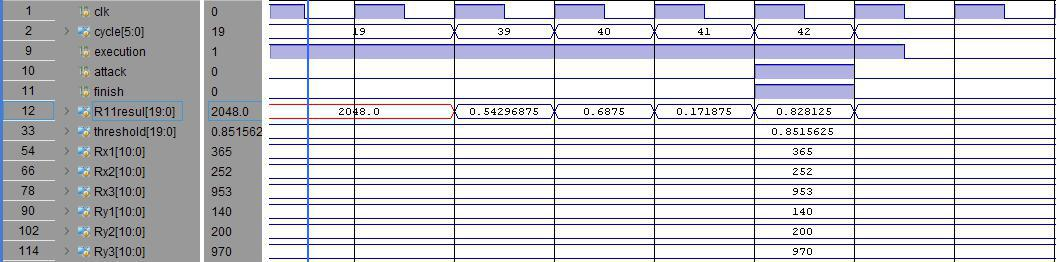
\includegraphics[width=14cm]{figures/simu.jpg}\\

		{Fonte: Elaborada pelo autor}
	
	\label{simu}
\end{figure}



\begin{table}[H]
	\centering
	\caption{Tempo de detecção}
	\label{Tab:TD}
	\begin{tabular}{lcccc}
		\hline
		\multicolumn{1}{c}{Detector}&\multicolumn{1}{c}{Artigo de comparação }&\multicolumn{1}{c}{Trabalho Proposto}&\multicolumn{1}{c}{Software(Matlab)}
		\\ \midrule
		
		Tempo de Detecção &  354 ns  &  350 ns & 296 $\mu$s  \\   \midrule
	
	\end{tabular}
\end{table}

A Tabela \ref{Tab:TD} mostra que existe um pequeno ganho de desempenho de aceleração, desse trabalho em relação ao artigo de comparação (também implementado em hardware), e obviamente um ganho significativo em relação ao detector em software.

